\documentclass[10pt]{article}
\usepackage[english]{babel}
\usepackage{amsmath, amsthm, amssymb, mathtools, thmtools, mathdots, tikz, mathrsfs}
%\usepackage{enumerate} conflicts with enumitem
\mathtoolsset{showonlyrefs}
\usepackage[shortlabels]{enumitem}
\usepackage{subcaption}
\usepackage{fancyhdr}
\usepackage{graphicx}
\usepackage{hyperref}
%\usepackage{parskip}
\usepackage[left=0.8in,top=0.8in,right=0.8in,bottom=0.8in]{geometry}
%\setlength{\headheight}{15.2pt}
%\setlength{\parindent}{0pt}
%\setlength{\parskip}{5pt}
\usepackage{indentfirst}
 \usepackage{hyperref}
\newcommand{\eat}[1]{}

%\usetikzlibrary{positioning,matrix}
\usetikzlibrary{shapes}

\hypersetup{colorlinks=true,linkcolor=blue,citecolor=gray}
\addto\extrasenglish{
    \renewcommand{\sectionautorefname}{Section}
    \renewcommand{\subsectionautorefname}{Section}
    \renewcommand{\subsubsectionautorefname}{Section}
}
% comment out the outer \addto\extrasenglish braces if not using babel package



%%%%%%%%%%%%%%%%%%%%%%%%%%%%%%%%%%%%%%%%%%%%%%%%%%%%%%%%%%%%%%%%%%%%%
\declaretheoremstyle[
    shaded={rulecolor={rgb}{0,0,0}, rulewidth=0.5pt, bgcolor={rgb}{1,1,1}}
]{boxedstyle}

\declaretheorem[name={Theorem}, style=boxedstyle, numberwithin=section]{thm}
\declaretheorem[name={Lemma}, style=boxedstyle, sibling=thm]{lem}
\declaretheorem[name={Proposition}, style=boxedstyle, sibling=thm]{prop}
\declaretheorem[name={Corollary}, style=boxedstyle, sibling=thm]{cor}
\declaretheorem[name={Problem}, sibling=thm]{prob}
\declaretheorem[name={Definition}, style=definition, sibling=thm, qed=$\blacksquare$]{df}
\declaretheorem[name={Example}, style=definition, sibling=thm, qed=$\blacksquare$]{example}

%%%%%%%%%%%%%%%%%%%%%%%%%%%%%%%%%%%%%%%%%%%%%%%%%%%%%%%%%%%%%%%%%%%%%

\title{When Variational Auto-encoders meet Generative Adversarial Networks}
\date{14 December 2016}
\author{Jianbo Chen\quad Billy Fang\quad Cheng Ju}

%%%%%%%%%%%%%%%%%%%%%%%%%%%%%%%%%%%%%%%%%%%%%%%%%%%%%%%%%%%%%%%%%%%%%

%\fancyhf{}
%\fancyhf[HL]{\sc{Billy Fang}}
%\fancyhf[HR]{\rightmark}
%\fancyhf[FC]{\thepage}

%%%%%%%%%%%%%%%%%%%%%%%%%%%%%%%%%%%%%%%%%%%%%%%%%%%%%%%%%%%%%%%%%%%%%
%\newcommand{\m}[1]{\mathcal{#1}}
%\renewcommand{\b}[1]{\mathbb{#1}}
\DeclarePairedDelimiter{\parens}{(}{)}
\DeclarePairedDelimiter{\braces}{\{}{\}}
\DeclarePairedDelimiter{\brackets}{[}{]}
\DeclarePairedDelimiter{\abs}{|}{|}
\DeclarePairedDelimiter{\norm}{\|}{\|}
\DeclarePairedDelimiter{\ceil}{\lceil}{\rceil}
\DeclarePairedDelimiter{\floor}{\lfloor}{\rfloor}
\DeclarePairedDelimiter{\inner}{\langle}{\rangle}
\DeclareMathOperator*{\argmin}{\arg\!\min}
\DeclareMathOperator*{\argmax}{\arg\!\max}
%\DeclareMathOperator{\im}{im}
%\DeclareMathOperator{\Aut}{Aut}
%\DeclareMathOperator{\Inn}{Inn}
%\DeclareMathOperator{\lcm}{lcm}
%\DeclareMathOperator{\trace}{trace}
%\DeclareMathOperator{\Hom}{Hom}
\newcommand{\op}[1]{\operatorname{#1}}
\renewcommand{\b}[1]{\boldsymbol{\mathbf{#1}}}
\renewcommand{\bar}[1]{\overline{#1}}
\renewcommand{\hat}[1]{\widehat{#1}}
\renewcommand{\tilde}[1]{\widetilde{#1}}
\newcommand{\E}{\mathbb{E}}
\renewcommand{\P}{\mathbb{P}}
\newcommand{\Var}{\op{Var}}
\newcommand{\Cov}{\op{Cov}}
\newcommand{\R}{\mathbb{R}}
\newcommand{\N}{\mathbb{N}}
\newcommand{\indep}{\mathop{\rotatebox[origin=c]{90}{$\models$}}}

%%%%%%%%%%%%%%%%%%%%%%%%%%%%%%%%%%%%%%%%%%%%%%%%%%%%%%%%%%%%%%%%%%%%%

%\renewcommand{\familydefault}{\sfdefault}
\DeclareTextFontCommand{\emph}{\bfseries}
%\usepackage{mathptmx}
%\renewcommand{\rmdefault}{ptm}
%\usepackage[default,scale=0.9]{opensans}

\allowdisplaybreaks[1]
\sloppy

%%%%%%%%%%%%%%%%%%%%%%%%%%%%%%%%%%%%%%%%%%%%%%%%%%%%%%%%%%%%%%%%%%%%%


\begin{document}

\maketitle


\begin{abstract}
Variational auto-encoders are a promising class of generative models. In this project, we first review variational auto-encoders (VAE) and its popular variants including the Conditional VAE \cite{sohn2015learning}, VAE for semi-supervised learning \cite{DBLP:journals/corr/KingmaRMW14} and DRAW \cite{chung2015recurrent}. We also investigate various applications of variational auto-encoders.
Finally, we propose models which combine variants of VAE with another popular deep generative model: generative adversarial networks \cite{goodfellow2014gan}, generalizing the idea proposed in \cite{larsen2015autoencoding}.
\end{abstract}


\section{Introduction}
Unsupervised learning from large unlabeled datasets is an active research area.
In practice, millions of images and videos are unlabeled and one can leverage them to learn good intermediate feature representations via approaches in unsupervised learning, which can then be used for other supervised or semi-supervised learning tasks such as classification.
One approach for unsupervised learning is to learn a generative model.
Two popular methods in computer vision are variational auto-encoders (VAEs) \cite{kingma2013auto} and generative adversarial networks (GANs) \cite{goodfellow2014gan}.

Variational auto-encoders are a class of deep generative models based on variational methods. %There exist many variants including conditional VAEs \cite{doersch2016tutorial}, VAEs tailored for semi-supervised learning \cite{DBLP:journals/corr/KingmaRMW14}, attention-based generative models \cite{gregor2015draw}, and more.
With sophisticated VAE models, one can not only generate realistic images, but also replicate consistent ``style.'' For example, DRAW \cite{gregor2015draw} was able to generate images of house numbers with number combinations not seen in the training set, but with a consistent style/color/font of street sign in each image. Additionally, as models learn to generate realistic output, they learn important features along the way, which potentially can be used for classification; we consider this in the Conditional VAE and semi-supervised learning models.
However, one main criticism of VAE models is that their generated output is often blurry.

Generative adversarial networks are another class of deep generative models. GANs introduce a game theoretic component to the training process, in which a discriminator learns to distinguish real images from generated images, while at the same time the generator learns to fool the discriminator.

In this report, we make the following contributions:
\begin{itemize}
\item We do a survey on the currently popular variants of variational auto-encoders and implement them in TensorFlow.
\item Based on previous work \cite{larsen2015autoencoding}, we combine popular variants of variational auto-encoders with generative adversarial networks, addressing the problem of blurry images.
\item We investigate a few applications of generative models, including image completion, style transfer and semi-supervised learning.
\end{itemize}

On the one hand, we were able to generate less blurry images by combining the Conditional VAE with a GAN, compared to the original Conditional VAE \cite{sohn2015learning}.
%and we successfully applied the conditional VAE to image completion and style transfer.
On the other hand, we did not get comparable accuracy in semi-supervised learning when we tried to combine VAE with GAN. DRAW yields strange results when combined with GAN. These problems and their potential solutions are detailed in section 5.



%This paragraph is very good. But I can't find a place to fit it in logically? Maybe separate it into various places?
%One obvious feature of generative models is their ability to produce realistic images and other output. With sophisticated models, one can even replicate consistent ``style.'' For example, DRAW \cite{gregor2015draw} was able to generate images of house numbers with number combinations not seen in the training set, but with a consistent style/color/font of street sign in each image. Additionally, as models learn to generate realistic output, they learn important features along the way, which potentially can be used for classification; we consider this in the conditional VAE and semi-supervised learning models.

% As we implement known models, we also explore generalizations and modifications. We have considered modifying the architecture of the various networks and modifying the various ways one can incorporate side data in the conditional VAE and semi-supervised settings.
%, as well as considering non-isotropic Gaussian models (which the current literature eludes).

%Since we are currently at an implementation/exploratory stage, we have not rigorously evaluated the quality of our gener{}ated output, but we intend to be more quantitative in this regard later on. As there is not a widely used quantitative metric for evaluating generative models, it is hard to state what the state-of-the-art model is; functionally, we will consider the models in the papers cited above to be the state-of-the-art, and we hope to improve on them by considering modifications/generalizations of these models.

 % To attempt to remedy this issue we add generative adversarial networks (GANs) to our models.



\section{Overview of VAE models}

\subsection{Variational auto-encoders}

In the \emph{variational auto-encoder (VAE)}  literature, we consider the following latent variable model for the data $x$.
\begin{align}
z &\sim \mathcal{N}(0,I)\\
x \mid z &\sim f(x ; z, \theta).
\end{align}
Here, $f(x;z,\theta)$ is some distribution parameterized by $z$ and $\theta$. In our work, we mainly consider $x \mid z$ being [conditionally] independent Bernoulli random variables (one for each pixel) with parameters being some function of the latent variable $z$ and possibly other parameters $\theta$.

We omit motivation of the variational approach, which is explained in more detail in \cite{doersch2016tutorial}.
We consider the following lower bound, valid for any distribution $Q(z \mid x)$.
\begin{equation}
\log p(x)
\ge \E_{z \sim Q(\cdot \mid x)}[\log p(x \mid z)]
- \op{KL}(Q(z \mid x) \| p(z)) =: -\mathcal{L}(x).
\label{equation:vae_loss}
\end{equation}
%We have equality if $Q(z \mid x)$ is precisely the posterior $p(z \mid x)$.
%Therefore, computing the posterior is just as hard as maximizing the likelihood.
In variational inference, we would maximize the right-hand side over a family of distributions $Q(z \mid x)$. Here we restrict our attention to $Q(z \mid x)$ being Gaussian with some mean $\mu(x)$ and diagonal covariance $\Sigma(x)$ being functions (namely, neural networks) of $x$.
For the VAE framework however, we also learn $p(x \mid z) = f(x;z,\theta)$; this too, is a neural network.

The VAE model is trained by maximizing the right-hand side of \eqref{equation:vae_loss}, and the structure is depicted in \autoref{figure:vae_model}. The first neural network, called the encoder, takes in the data $x$ and outputs the mean $\mu(x)$ and variance $\Sigma(x)$ of $Q(z \mid x)$, which then can be used to compute the KL-divergence term in the loss. We then sample $z \sim Q(z \mid x)$ by computing $\Sigma(x)\cdot \epsilon + \mu(x)$ where $\epsilon \sim \mathcal{N}(0,I)$, and pass $z$ through the second neural network, called the decoder, which allows us to compute $p(x \mid z)$. Since $z \sim Q(z \mid x)$, this is an unbiased estimate of $\mathbb{E}_{z \sim Q(\cdot \mid x)} [\log p(x \mid z)]$.


\begin{figure}[!ht]
\centering
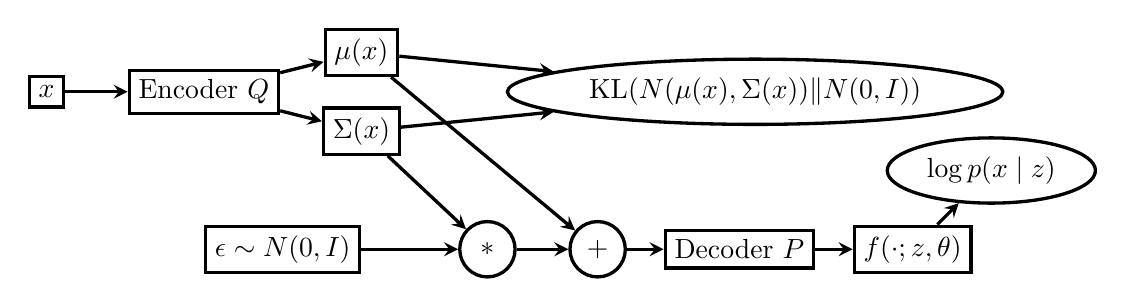
\begin{tikzpicture}[rectangle, ->,>=stealth,very thick,scale=2]
\node[draw] (X) at (0,0) {$x$};
\node[draw] (enc) at (1,0) {Encoder $Q$};
\node[draw] (mu) at (2,0.25) {$\mu(x)$};
\node[draw] (sigma) at (2,-0.25) {$\Sigma(x)$};
\node[draw] (eps) at (1.5,-1) {$\epsilon \sim N(0,I)$};
\node[circle, draw, minimum size = 2em] (times) at (2.8,-1) {$*$};
\node[circle, draw, minimum size = 2em] (plus) at (3.5,-1) {$+$};
\node[draw] (dec) at (4.4,-1) {Decoder $P$};
\node[draw] (f) at (5.5,-1) {$f(\cdot; z, \theta)$};
\node[ellipse, draw] (kl) at (4.5,0) {$\op{KL}(N(\mu(x),\Sigma(x))\| N(0,I))$};
\node[ellipse, draw] (decloss) at (6,-0.5) {$\log p(x \mid z)$};
%\node (decloss_lab) at (4,-0.5) {decoder loss/reconstr. error};
%\node (encloss_lab) at (4.5,0.5) {encoder loss/regularization};
\draw (X) to (enc);
\draw (enc) to (mu);
\draw (enc) to (sigma);
\draw (eps) to (times);
\draw (times) to (plus);
\draw (sigma) to (times);
\draw (mu) to (plus);
\draw (plus) to (dec);
\draw (dec) to (f);
\draw (mu) to (kl);
\draw (sigma) to (kl);
\draw (f) to (decloss);
\end{tikzpicture}
\caption{Variational auto-encoder structure.}
\label{figure:vae_model}
\end{figure}

To generate new data, we simply sample $z \sim \mathcal{N}(0,I)$ and input it into the trained decoder.
More information can be found in the original paper \cite{kingma2013auto} as well as in the tutorial \cite{doersch2016tutorial}.


\subsection{Conditional variational auto-encoders}

One variant of the VAE is the \emph{Conditional variational auto-encoder (CVAE)} \cite{sohn2015learning}, which makes use of side information $y$, such as a label or part of an image. Mathematically the variational approach is the same as above except with conditioning on $y$.
\begin{equation}
\log p(x \mid y)
\ge \E_{z \sim Q(\cdot \mid y,x)}[\log p(x \mid y,z)]
- \op{KL}(Q(z \mid x,y) \| p(z \mid y))=: -\mathcal{L}(x,y).
\end{equation}
The CVAE structure appears in \autoref{figure:cvae_model}. Structurally, the only difference is that both the encoder and decoder take the side information $y$ as extra input.

\begin{figure}[!ht]
\centering
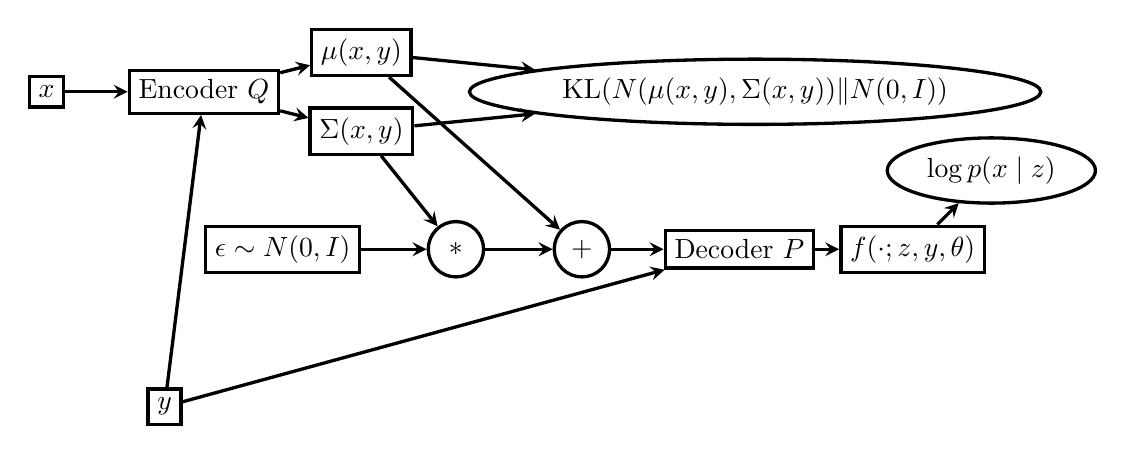
\begin{tikzpicture}[rectangle, ->,>=stealth,very thick,scale=2]
\node[draw] (Y) at (0.75,-2) {$y$};
\node[draw] (X) at (0,0) {$x$};
\node[draw] (enc) at (1,0) {Encoder $Q$};
\node[draw] (mu) at (2,0.25) {$\mu(x,y)$};
\node[draw] (sigma) at (2,-0.25) {$\Sigma(x,y)$};
\node[draw] (eps) at (1.5,-1) {$\epsilon \sim N(0,I)$};
\node[circle, draw, minimum size = 2em] (times) at (2.6,-1) {$*$};
\node[circle, draw, minimum size = 2em] (plus) at (3.4,-1) {$+$};
\node[draw] (dec) at (4.4,-1) {Decoder $P$};
\node[draw] (f) at (5.5,-1) {$f(\cdot;z,y,\theta)$};
\node[ellipse, draw] (kl) at (4.5,0) {$\op{KL}(N(\mu(x,y),\Sigma(x,y))\| N(0,I))$};
\node[ellipse, draw] (decloss) at (6,-0.5) {$\log p(x \mid z)$};
\draw (X) to (enc);
\draw (enc) to (mu);
\draw (enc) to (sigma);
\draw (eps) to (times);
\draw (times) to (plus);
\draw (sigma) to (times);
\draw (mu) to (plus);
\draw (plus) to (dec);
\draw (dec) to (f);
\draw (mu) to (kl);
\draw (sigma) to (kl);
\draw (f) to (decloss);
\draw (Y) to (enc);
\draw (Y) to (dec);
\end{tikzpicture}
\caption{Conditional variational auto-encoder structure}
\label{figure:cvae_model}
\end{figure}

At generation time, we input not only a fresh sample $z \sim \mathcal{N}(0,I)$, but also some side information $y$ into the decoder. We explore different examples of side information in \autoref{sub:cvae_app}.
\subsection{Semi-supervised learning}
Kingma et al. \cite{DBLP:journals/corr/KingmaRMW14} introduced a variant of the VAE framework tailored for semi-supervised learning (SSL), where the goal is classification after training on a dataset that has both labeled and unlabeled examples. Unlike the CVAE where everything was conditioned on the label $y$, the SSL model gives $y$ a categorical distribution. The generative model (called ``M2'' in \cite{DBLP:journals/corr/KingmaRMW14}) is as follows.
\begin{align}
y &\sim \op{Cat}(\pi)\\
z &\sim \mathcal{N}(0,I)\\
x \mid y,z &\sim f(x; y,z,\theta)
\end{align}

We maximize a lower bound on the log likelihood (of both the data $x$ and the label $y$) over normal distributions $Q(z \mid x,y)$ and categorical distributions $Q(y \mid x)$. However, for unlabeled examples, we marginalize over $y \sim q(y \mid x)$. This gives us the labeled and unlabeled losses $\mathcal{L}(x,y)$ and $\mathcal{U}(x)$ below.
\begin{align}
\log p(x,y)
&\ge \E_{z \sim Q(z \mid x,y)}[\log p(x \mid y,z) + \log p(y)] - \op{KL}(Q(z \mid x,y) \| p(z)) =: - \mathcal{L}(x,y)\\
\log p(x) &\ge \sum_y Q(y \mid x) (-\mathcal{L}(x,y)) + H(Q(y \mid x)) =: -\mathcal{U}(x).
\end{align}

\begin{figure}[!ht]
\centering
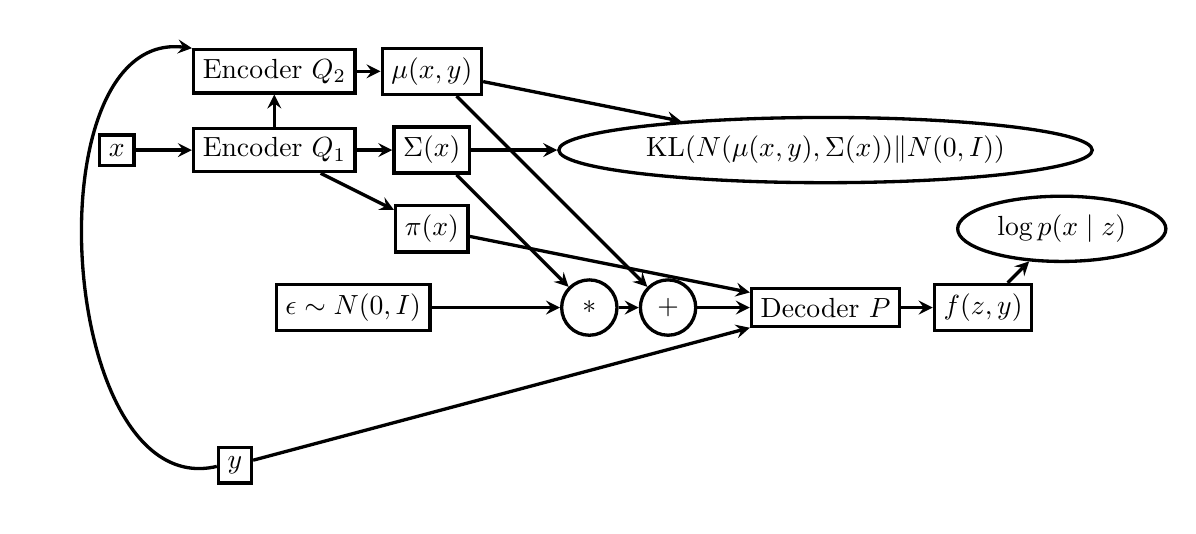
\begin{tikzpicture}[rectangle, ->,>=stealth,very thick,scale=2]
\node[draw] (Y) at (0.75,-2) {$y$};
\node[draw] (X) at (0,0) {$x$};
\node[draw] (enc) at (1,0) {Encoder $Q_1$};
\node[draw] (enc2) at (1,0.5) {Encoder $Q_2$};
\node[draw] (mu) at (2,0.5) {$\mu(x,y)$};
\node[draw] (sigma) at (2,0) {$\Sigma(x)$};
\node[draw] (pi) at (2,-0.5) {$\pi(x)$};
\node[draw] (eps) at (1.5,-1) {$\epsilon \sim N(0,I)$};
\node[circle, draw, minimum size = 2em] (times) at (3,-1) {$*$};
\node[circle, draw, minimum size = 2em] (plus) at (3.5,-1) {$+$};
\node[draw] (dec) at (4.5,-1) {Decoder $P$};
\node[draw] (f) at (5.5,-1) {$f(z,y)$};
\node[ellipse, draw] (kl) at (4.5,0) {$\op{KL}(N(\mu(x,y),\Sigma(x))\| N(0,I))$};
\node[ellipse, draw] (decloss) at (6,-0.5) {$\log p(x \mid z)$};
\draw (X) to (enc);
%\draw (enc) to (mu);
\draw (enc) to (sigma);
\draw (eps) to (times);
\draw (times) to (plus);
\draw (sigma) to (times);
\draw (mu) to (plus);
\draw (plus) to (dec);
\draw (dec) to (f);
\draw (mu) to (kl);
\draw (sigma) to (kl);
\draw (f) to (decloss);
\draw (Y) to [bend left =100] (enc2);
\draw (Y) to (dec);
\draw (enc) to (pi);
\draw (enc2) to (mu);
\draw (pi) to (dec);
%\draw (X) to (enc2);
\draw (enc) to (enc2);
\end{tikzpicture}
\caption{Model for semi-supervised learning}
\label{figure:ssl_model}
\end{figure}

The total loss is
\begin{equation}
\sum_{\text{labeled $(x,y)$}} \mathcal{L}(x,y)
+ \sum_{\text{unlabeled $x$}} \mathcal{U}(x).
\end{equation}
In \cite{DBLP:journals/corr/KingmaRMW14}, they also add an extra classification loss $\alpha \mathbb{E}_{\text{labeled $(x,y)$}}[-\log Q(y \mid x)]$ so that the predictive distribution $q(y \mid x)$ also contributes to $\mathcal{L}(x,y)$.

We can use this for labeled image generation as before: input $z \sim \mathcal{N}(0,I)$ and $y$ into the decoder.

For classification, we input the unlabeled image into the decoder and return the class with the highest probability according to the categorical distribution parameterized by $\pi(x)$.

\subsection{DRAW}

The Deep Recurrent Attentive Writer (DRAW) \cite{gregor2015draw} is an extension of the vanilla variational auto-encoder generator.
It applies the sequential variational auto-encoding framework to iteratively construct complicated images, with a soft attention mechanism.
There are three main differences between the DRAW and vanilla VAE.
\begin{enumerate}
    \item Both the encoder and decoder of DRAW are recurrent networks.
    \item The decoder’s outputs are successively added to the distribution that will ultimately generate the data (image), as opposed to emitting this distribution in a single step.
    \item A dynamically updated attention mechanism is used in DRAW to restrict the input region observed by the encoder, which is computed by the previous decoder.
\end{enumerate}

\begin{figure}[!ht]\centering
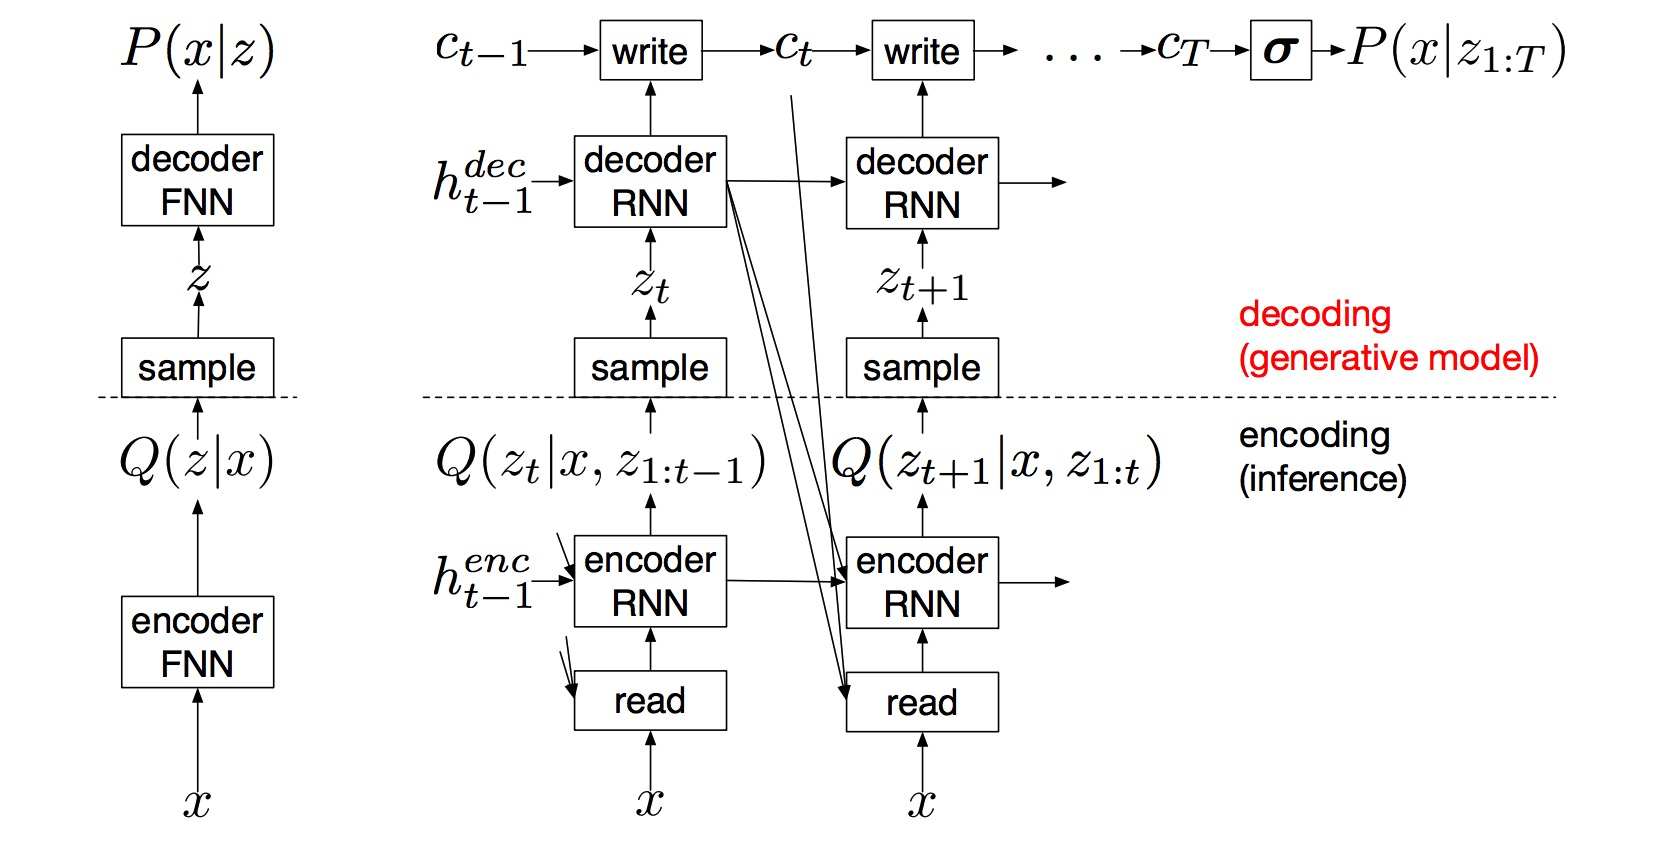
\includegraphics[width=0.5\textwidth]{images/draw_structure.png}
\caption{Conventional Variational Auto-Encoder (left) and DRAW Network \cite{gregor2015draw} (right)}
\label{figure:draw_structure}
\end{figure}

\autoref{figure:draw_structure} shows the structure of DRAW. The input for each encoder cell is convoluted image, where the convolution is computed by the previous decoder cell. Thus the input for each encoder is dynamically computed.

The loss comes from two parts. The decoder loss is the same as the vanilla VAE: only the final canvas matrix (which is the cumulative sum of the previous decoder output) is used to compute the distribution of the data $D(x|c_T)$. If the input is binary, the natural choice for D is a Bernoulli distribution with means given by $\sigma(c_T)$, and the reconstruction loss is the negative log probability of $x$ under $D$:

$$L^{x} = - \log D(x|c_T)$$

The encoder loss is different. DRAW uses cumulative Kullback-Leibler divergence across time $T$ as the encoder loss:

$$L^z = \sum_{t=1}^{T} KL(Q(Z_t|h_{t}^{enc})||Z_t) = \frac{1}{2}\sum_{t=1}^{T}(\mu_t^2 + \sigma_t^2 - \log \sigma^2_t) - T/2$$

The total loss L for the network is the expectation of the sum of the reconstruction and latent losses:
$$L = \E_{z \sim Q} (L^z + L^x).$$

Conditional DRAW is an extension of vanilla DRAW analogous to the CVAE described above. The input of the encoder and decoder of conditional DRAW is the same as vanilla DRAW, except with additional information (e.g. the label of the image).







\section{Combining generative adversarial networks with VAEs}

In this section, we investigate how we can combine various variants of VAEs reviewed above with another popular generative model: generative adversarial networks (GANs) \cite{goodfellow2014gan}. In a GAN, a generator and a discriminator are trained together.
The discriminator is trained to distinguish ``real'' images from ``fake'' (i.e. generated), while the generator is trained to generate images that the discriminator will classify as ``real.''
Abstractly, combining the GAN framework with VAEs is straightforward: the generator in the GAN framework is the VAE. Below we discuss the details and our results for various variants of VAEs.

\subsection{VAE with GAN}
The basic idea is the following: Let $D(x)$ denote the output of the discriminator for an image $x$; this represents the probability that $x$ is a real image. As in GAN, we train the generator (which is a VAE here) and the discriminator alternately, by minimizing two losses separately.

The generator loss is formed by adding an extra term $-\log D(\op{Dec}(z))$, which punishes the generated images being classified as fake. The discriminator loss is $-\log D(x) - \log (1-D(\op{Dec}(z))$, the same as in a pure GAN.

Based on ideas in \cite{larsen2015autoencoding}, we make the following two modifications on the simplified model:
\begin{itemize}
\item Replacing the VAE decoder/reconstruction loss $\mathbb{E}_{z \sim Q(\cdot \mid x)} \log p(x \mid z)$ with a dissimilarity loss $\mathcal{L}_{llike}^{\op{Dis}_l}$ based on the $l$th layer inside the discriminator. That is, we input both the original image $x$ and a generated image $\op{Dec}(z)$ into the discriminator, and use the $L^2$ distance between the output of the $l$th layer of the discriminator as the decoder loss (this can be interpreted as maximizing the log likelihood of a Gaussian distribution) instead of the original pixel-based loss. The intuition is that the deeper layers of the discriminator will learn good features of the images, and that using this as the decoder/reconstruction loss will be more informative than using a pixel-based loss. Mathematically, the reconstruction loss is a $l_2$ loss:
$$
\mathcal{L}_{llike}^{\op{Dis}_l} = \|f_l(x) - f_l(\tilde{x})\|^2 / 2\sigma^2 +Const.
$$
where $f_l(x)$ is the result of $x$ passing through the $l$th layer of the discriminator network, and $\tilde x$ is the result getting from letting $x$ pass through the encoder and then the decoder.

\item Incorporate the classification of the reconstructed image $\op{Dec}(\op{Enc}(x))$ by adding $-\log D(\op{Dec}(\op{Enc}(x)))$ and $-\log (1-D(\op{Dec}(\op{Enc}(x)))))$ to the VAE and discriminator losses respectively. Since the reconstructed image is close to the original image, this will help train the discriminator.
\end{itemize}

In summary, the generator loss is
\begin{equation}\label{vaegan1}
L_G = \mathcal{L}_{KL} + \mathcal{L}_{llike}^{\op{Dis}_l} -\log D(\op{Dec}(z)) -\log D(\op{Dec}(\op{Enc}(x)))
\end{equation}
where $z$ is generated from the prior $p(z)$ of latent variables ($p(z) = \mathcal{N}(0,I)$) and $\mathcal{L}_{KL} = KL(q(z|x),p(z))$ is the same as the regularization term in VAE.
The discriminator loss is
\begin{equation}\label{vaegan2}
L_D = -\log D(x) - \log (1-D(\op{Dec}(z)) -\log (1-D(\op{Dec}(\op{Enc}(x)))),
\end{equation}
where $z$ is generated from the prior of latent variables ($N(0,I)$).

The structure of the model is shown in \autoref{figure:vaegan_model} \cite{larsen2015autoencoding}.

\begin{figure}[!ht]\centering
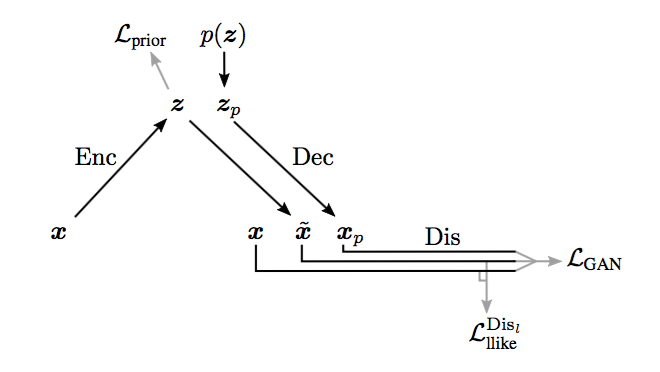
\includegraphics[width=0.5\textwidth]{images/vaegan2.png}
\caption{VAE with GAN model from \cite{larsen2015autoencoding}}
\label{figure:vaegan_model}
\end{figure}

\subsection{CVAE with GAN}
One generalization of VAE with GAN is to incorporate the side information $y$, such as a label or part of an image. Our idea is to put a GAN on top of a Conditional VAE. To make full use of the side information $y$, the structure of the discriminator of GAN is also modified. Suppose $y$ is a label which has $k$ classes. Then the discriminator $D$ outputs a distribution on $k+1$ classes. We wish the discrimator to assign the correct label among $k$ classes for a true example $(x,y)$ but assign generated images to the extra $k+1$th class. Formally, define $D$ as a function from the image space to a distribution on $k+1$ classes:
$$
\sum_{c=1}^{k+1} D_c(x) = 1, D_c(x) \geq 0.
$$
We still train the generator and the discriminator alternately. The generator loss is formed as a sum of the loss of a Conditional VAE and the loss from GAN which is a cross entropy loss over the output of the discriminator which punishes generated images for being classified into a wrong class. The mathematical representation is shown below. Recall that the encoder and the decoder of a conditional VAE both take $y$ as an input.
The cross entropy loss takes as input a distribution $p$ on classes and a label $y$, and outputs $-\log p(Y=y)$.
\begin{align}
L_G &= \mathcal{L}_{KL} + \mathcal{L}_{llike}^{\op{Dis}_l} \\
&\qquad +CrossEntropy(D(\op{Dec}(z,y)),y)\\
&\qquad +CrossEntropy(D(\op{Dec}(\op{Enc}(x,y),y),y),
\end{align}
where $z$ is generated from the prior $p(z)$ of latent variables. $\mathcal{L}_{KL}$ and $\mathcal{L}_{llike}^{\op{Dis}_l}$ are exactly the same as those in the previous section, except that we also feed in $y$ when generating images from the decoder.

The discriminator loss is a cross entropy loss over the output of the discriminator which punishes classifying a real image into a wrong class or classifying a generated image into the first $k$ classes. Concretely, the discriminator loss is
\begin{align}
L_D &= CrossEntropy(D(x),y)\\
&\qquad + CrossEntropy(D(\op{Dec(z,y)}),y_{fake})\\
&\qquad +CrossEntropy(D(\op{Dec(Enc(x,y),y)}),y_{fake}),
\end{align}
where $z$ is generated from the prior of latent variables and $y_{fake}$ is the label for the extra $(k+1)$st class.


\subsection{SSL with GAN}
The VAE tailored for semi-supervised learning (SSL) can also be incorporated with a $k+1$-class GAN in a similar way as CVAE. Recall that the VAE-SSL loss is divided into two parts: a loss for labeled data and a loss for unlabeled data. The method of incorporating GAN to VAE-SSL is exactly the same as that of CVAE for labeled data; refer to the previous section for details. For unlabeled data, recall that the VAE loss is
$$
\sum_y Q(y \mid x) (-\mathcal{L}(x,y)) + H(Q(y \mid x)) =: -\mathcal{U}(x),
$$
where a categorical distribution $Q(y|x)$ is introduced. We mimic the idea that when a label $y$ is needed as an input, the loss is averaged over $Q(y|x)$. Mathematically:
\begin{align}
L_{G,unobserved} &= \mathcal{L}_{KL} + H(Q(y|x))+\sum_y Q(y|x)\Big(\mathcal{L}_{llike}^{\op{Dis}_l} \\
&\qquad +CrossEntropy(D(\op{Dec}(z,y)),y)\\
&\qquad +CrossEntropy(D(\op{Dec}(\op{Enc}(x,y),y),y)\Big),
\end{align}
where we emphasize that $\mathcal{L}_{llike}^{\op{Dis}_l}$ also depends on $y$ and needs to be averaged, and that the entropy term $H(Q(y|x))$ is introduced to regularize over $Q$ as before.
The discriminator loss is again averaged over $Q(y|x)$:
\begin{align}
L_D &= \sum_y Q(y|x)\big(CrossEntropy(D(x),y)\\
&\qquad + CrossEntropy(D(\op{Dec(z,y)}),y_{fake}) \\
&\qquad +CrossEntropy(D(\op{Dec(Enc(x,y),y)}),y_{fake})\big).
\end{align}
\subsection{DRAW with GAN}
Unlike the VAE, which only generates one image, DRAW generates a sequence of images.
Thus, there are two potential way to combine DRAW with GAN: we could either add discriminator on the top of all the temporary canvas, or only on the top of the last output.
In this project, we only consider the latter one.
If we consider DRAW as a black-box generator like the vanilla VAE, the structure is exactly the same as VAE-GAN.
The two losses that we minimize alternately take the same forms as \eqref{vaegan1} and \eqref{vaegan2}, but instead use the decoder and the encoder from DRAW.

\section{Experiments and Applications}
In the project, we implemented all the models mentioned above and studied their performance.
The code will be made available at \href{url}{https://github.com/Jianbo-Lab/vae-gan}.
In this section, we discuss details about the implementation, investigate applications of various models and compare the performances of various models.
All models were trained with mini-batch stochastic gradient descent (SGD) with a mini-batch size of $100$. All weights were initialized from a zero-centered Normal distribution. Batch-normalization \cite{sergey2015batchnorm} was added to all fully connected and convolutional layers except the output layers.
The Adam \cite{kingma2014adam} optimizer with default hyperparameters in TensorFlow was used for optimization. For various VAEs without GANs, we used the learning rate $0.001$ while for all VAEs with GANs, we use learning rate $0.0001$.
Due to the page limit, we omit the detailed description of our implementations of VAE-GAN. We refer interested readers to our GitHub repository for details.
\subsection{Tools}
We implemented all the models in TensorFlow. We used a GeForce GTX 770 GPU through Amazon for training. Git and Github were also very helpful for collaboration and managing our codebase.
\subsection{Dataset}
We used the MNIST handwritten digits dataset \cite{lecun1998gradient} through TensorFlow as well as the Street View House Numbers (SVHN) dataset \cite{netzer2011reading}. The MNIST dataset consists of a training dataset with $55,000$ labeled handwritten digits, a validation dataset with $5,000$ examples and a test set with $5,000$ examples. SVHN is a real-world image dataset similar in flavor to MNIST (e.g., the images are of small cropped digits), but incorporates an order of magnitude more labeled data (over $600,000$ digit images) and comes from a significantly harder, unsolved, real world problem (recognizing digits and numbers in natural scene images) \cite{netzer2011reading}.
We treated the MNIST images as a $28\times 28$-long vector with pixel values in $[0,1]$. We treated the SVHN images as a $32 \times 32 \times 3$-long vector with RGB values in $[0,1]$. No other data cleaning was needed.


\subsection{CVAE v.s. CVAE-GAN}
% Note that the VAE model in \autoref{figure:vae_model} does not incorporate labels at all, so we do not have explicit control on what digits we generate, unless we manually explore the latent space of $z$.

This experiment aims to compare the performance of CVAE with that of CVAE-GAN in terms of generating images. In this experiment, we feed into a trained decoder of CVAE a label ($1$ to $10$) and a randomly generated $z$ from the standard normal $\mathcal{N}(0,I)$. Then the corresponding handwritten digits will be generated according to the label. \autoref{figure:cvae_label} shows ten generated samples of each digit after training on MNIST and SVHN using CVAE. \autoref{figure:cvaegan_label} shows ten generated samples of each digit after training on MNIST and SVHN using CVAE with GAN.

The networks of CVAE and CVAE-GAN are constructed based on structures for DCGAN \cite{alec2016dcgan} with slight modification. In particular, we replace pooling by strided convolutions (discriminator) and fractional-strided convolutions (decoder) and remove all unnecessary fully connected layers (except at the outputs). Below we briefly describe the network structure of the encoder, the decoder and the discriminator (for MNIST), following notations used in class \cite{class}. The discriminator network is only used in CVAE-GAN while the encoder and the decoder networks are used both in CVAE and CVAE-GAN. Note that we use the same network structure for SVHN, except that the number of neurons at each layer increases by $8/7$.
\begin{itemize}
	\item Encoder:
  \[
   \left\{\begin{array}{lr}
        \text{Input } x:[28\times 28]\to \text{conv5-28} \to \text{conv5-56} &\to \text{conv5-108}\}\\
        &\text{Input } y:[10]
        \end{array}\right\} \to
        \left\{\begin{array}{lr}
        \text{FC-50}&\to \Sigma\\
        \text{FC-50}&\to \mu
        \end{array}\right\}
  \]

	\item Decoder:
\begin{align}
\text{Input } z \text{ concat with } y: [50 + 10] &\to \text{FC-7*7*128} \to \text{reshape}[7\times 7\times 128] \to \\
&\to \text{deconv5-64} \to \text{deconv5-32} \to \text{output } x:[28\times 28]
\end{align}
Here deconv is also called fractionally-strided convolutions in literature \cite{alec2016dcgan}.
\item Discriminator:
\[
\text{Input } x: [28\times 28] \to \text{conv3-16} \to \text{conv3-32} \to \text{conv3-64} \\
\to \text{FC-512} \to \left\{\begin{array}{lr}
        \text{FC-500}\to \text{Softmax}\\
        \text{$l$th layer $f_l(x)$}
        \end{array}\right\}
\]
\end{itemize}

\begin{figure}[!ht]
\centering
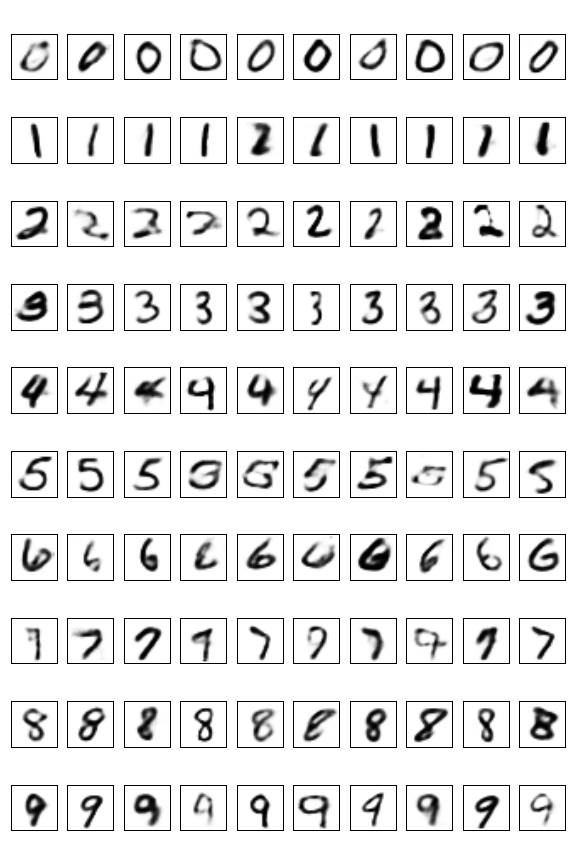
\includegraphics[width=0.35\textwidth]{images/by_label.png}
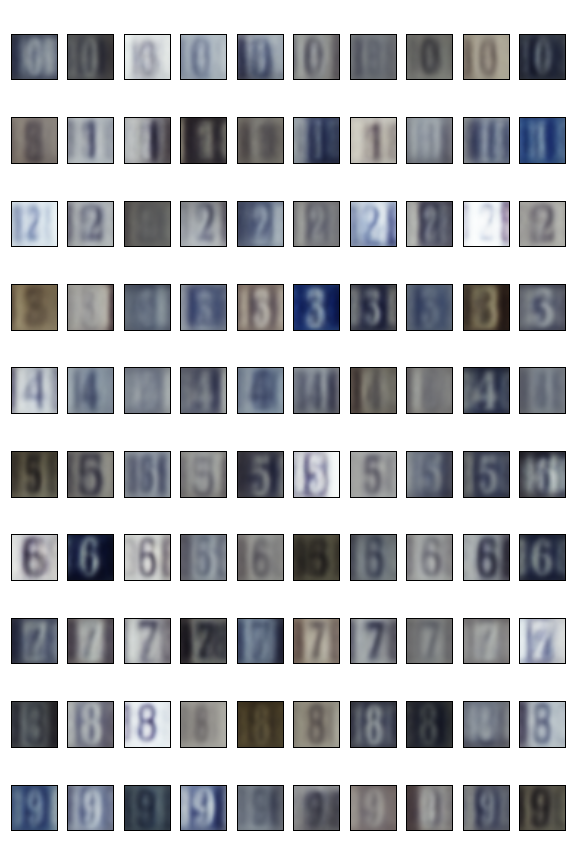
\includegraphics[width=0.35\textwidth]{images/svhn_cvae_fc_label_gen.png}
\caption{Purely generated images for MNIST (left) and SVHN (right) by CVAE. Since the CVAE incorporates labels into generation, we are able to generate a particular digit we choose.}
\label{figure:cvae_label}
\end{figure}

\begin{figure}[!ht]
\centering
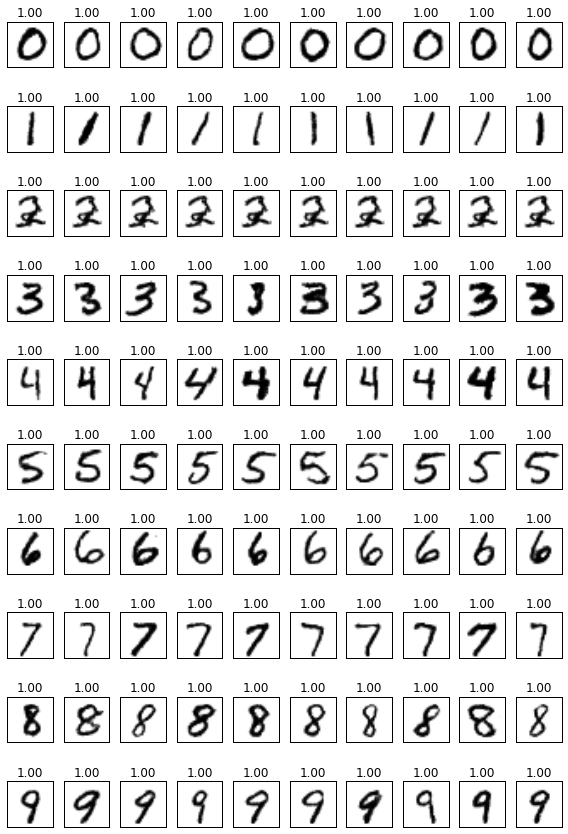
\includegraphics[width=0.35\textwidth]{images/cvaegan-mnist.png}
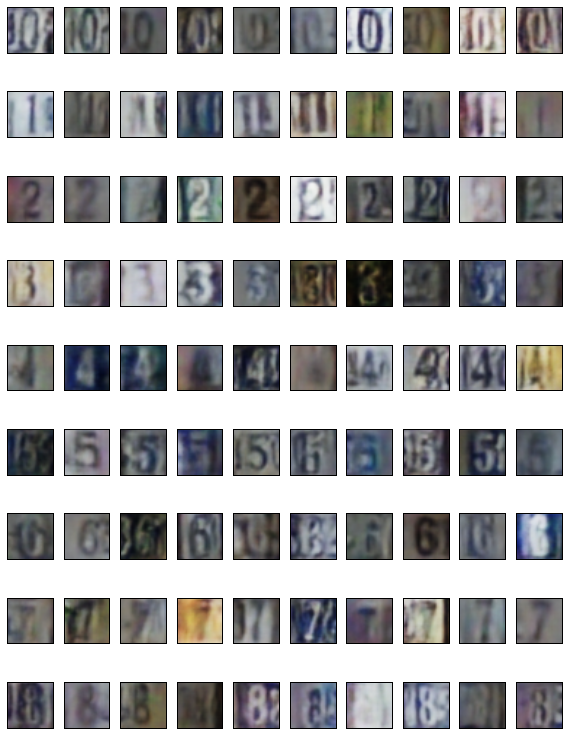
\includegraphics[width=0.35\textwidth]{images/cvaegan-svhn.png}
\caption{Purely generated images for MNIST (left) and SVHN (right) by CVAE-GAN.}
\label{figure:cvaegan_label}
\end{figure}
Comparing the results of CVAE and CVAE-GAN, we can see CVAE-GAN generates less blurry MNIST images compared to CVAE. But for the digit ``$2$,'' CVAE-GAN generates highly similar and strange images constantly. For the SVHN dataset, most of images generated by CVAE-GAN are less blurry, but there are also some weird images generated, like the digit ``$7$'' in the fourth column. We put the fixing of these problems to future work.
\subsection{CVAE applications}\label{sub:cvae_app}

% For our CVAE applications, we used a simple fully-connected architecture for a quick demonstration:
% \begin{itemize}
% \item Both the encoder and decoder are two-layer fully-connected neural networks with softplus activation. For MNIST, each layer has $200$ units; for SVHN each layer has $512$ units.
% \item The latent variable $z$ is $50$-dimensional.
% \end{itemize}
When implementing the CVAE model, we also investigated various applications of CVAE. In particular, we show here how we use a simple fully-connected CVAE for image completion and style transfer.
\subsubsection{Image completion}
The side information $y$ need not be a label. Here, we considered $y$ as being the left half of an image. At generation time, we can input a new half-image into the decoder, and it will attempt to complete the image based on what it has learned from the training data. Our demonstration appears in \autoref{figure:cvae_completion}.
\begin{figure}[!ht]
\centering
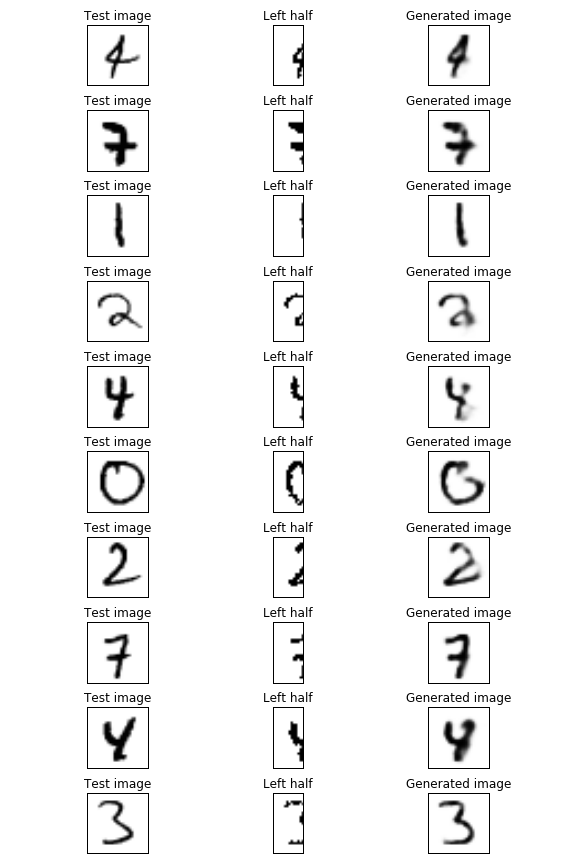
\includegraphics[width=0.35\textwidth]{images/left_half.png}
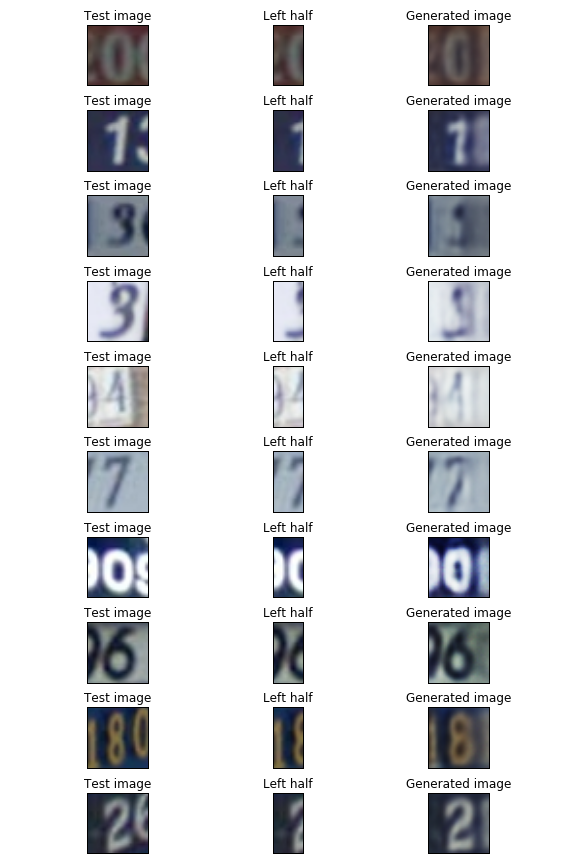
\includegraphics[width=0.35\textwidth]{images/svhn_left_half.png}
\caption{Image completion for MNIST (left) and SVHN (right). We take half-images from the test data and input them into the decoder, which attempts to complete the image based on what it has learned from the training data.}
\label{figure:cvae_completion}
\end{figure}

\subsubsection{Style transfer}
The CVAE can be used to transfer style from one image to the generated output. To do so, we input the base image (whose style we want to copy) into the encoder and obtain its latent ``code'' $z$. We then input this sampled $z$, which captures the features and style of the base image, along with an arbitrary label $y$ into the decoder. The output is then a digit with label $y$, but with the style of the original image. As shown in \autoref{figure:cvae_style}, we are able to copy boldness and slant in the case of MNIST, as well as font style, font color, and background color in the case of SVHN.
\begin{figure}[!ht]
\centering
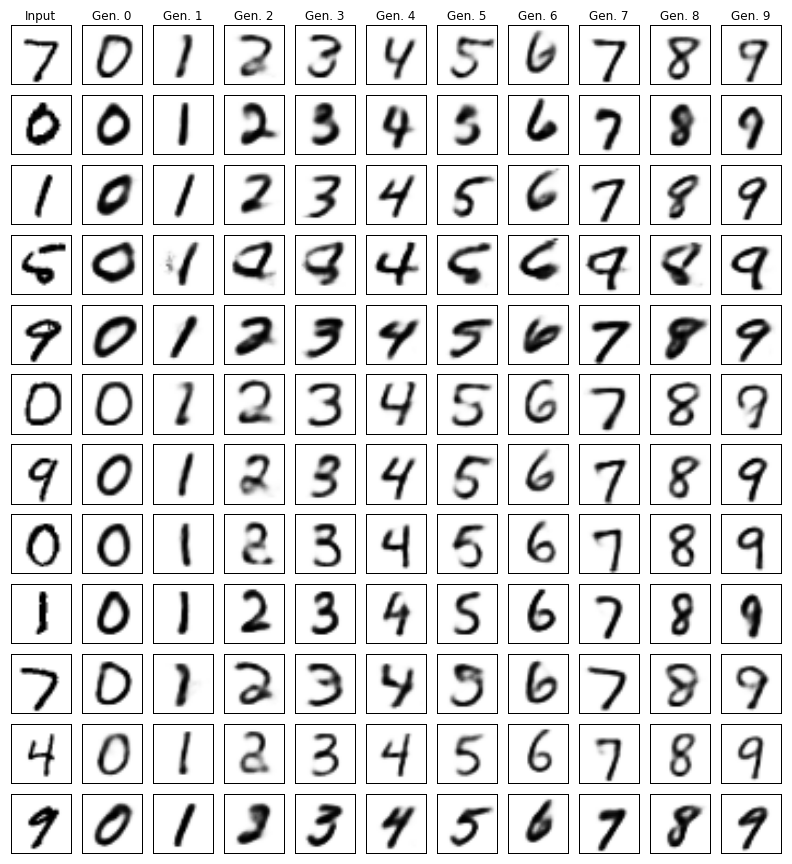
\includegraphics[width=0.45\textwidth]{images/style.png}
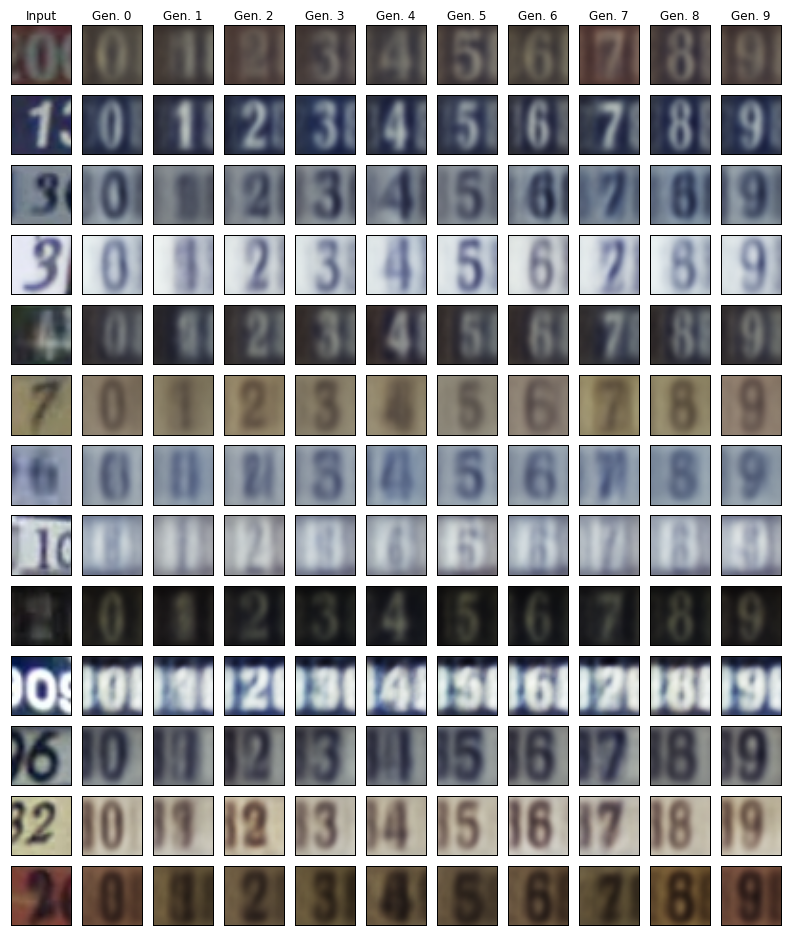
\includegraphics[width=0.45\textwidth]{images/svhn_cvae_fc_style.png}
\caption{Style transfer for MNIST (left) and SVHN (right). We transfer the style of the first column to all digits $0$ to $9$.}
\label{figure:cvae_style}
\end{figure}



\subsection{Semi-supervised learning}

This experiment compares the performance of VAE and that of VAE-GAN in semi-supervised learning. We followed the ``M2'' model of \cite{DBLP:journals/corr/KingmaRMW14} depicted in \autoref{figure:ssl_model}.

We took the $55000$ examples in the MNIST dataset and retained only $1000$ or $600$ of the labels (so that more than $98\%$ of the data is unlabeled!), with each label equally represented.

We considered both a fully-connected architecture and a convolutional architecture. For the discriminator of GAN, we still use the same structure as that of CVAE-GAN. Interested readers can refer to the previous section for details. Below we describe the network structures of the encoder and the decoder.
\begin{itemize}
	\item Fully connected
    \begin{itemize}
    	%\item For the first part of the encoder we used a three-layer fully-connected network, along with batch normalization and softplus activation to compute $\Sigma(x)$, $\pi(x)$ and another output that is then fed into the second part of the encoder which is a two-layer fully-connected network, and outputs $\mu(x,y)$.
        %\item The decoder has a three-layer fully-connected network.
        %\item Each hidden fully-connected layer has 1024 units.
        \item In the fully connected model described below, each hidden layer has batch normalization and softplus activation.
        \item Encoder:
        \begin{align}
            &\text{Input $x$: $[28 \times 28]$}:
            \to
            \text{FC-1024}
            \to
            \text{FC-1024}
            \to
            \begin{cases}
            h_1\\
            \text{FC-50} \to \Sigma(x)\\
            \text{FC-50} \to \pi(x)
            \end{cases}\\
            &\text{$h_1$ concat with $y$}: [1024+10] \to
            \text{FC-1024}
            \to
            \text{FC-50}
            \to
            \mu(x,y)
        \end{align}
        \item Decoder:
        \begin{equation}
        \text{Input $z$ concat with $y$: $[50+10]$}
        \to
        \text{FC-1024}
        \to
        \text{FC-1024}
        \to
        \text{FC-28*28-sigmoid}
        \to
        \text{output $x$: $[28 \times 28]$}
        \end{equation}
    \end{itemize}
    \item Convolutional model
    \begin{itemize}
    	\item For the convolutional version we replaced the hidden fully-connected layers with $5\times 5$ convolutions (in the encoder) and convolution transposes (``deconvolutions''). Below, all convolutions and deconvolutions have stride $1$. The argument of $\op{Conv}$ and $\op{Deconv}$ is the number of filters. $2\times 2$ max pooling and $2\times 2$ upsampling are denoted by $\Downarrow$ and $\Uparrow$ respectively.
        \item All layers have batch normalization except the output layers. All fully-connected layers have ReLU activation except the output layers.
        \begin{align}
        Q_1:& \quad x,\op{Conv}(20), \Downarrow, \op{Conv}(50), \Downarrow, \op{FC}(1024), \{\text{FC for $\Sigma$, FC-sigmoid for $\pi$}\}\\
        Q_2:& \quad (x,y), \op{FC}(1024), \op{FC}\\
        P:& \quad z,\op{FC}(500),\op{FC}(7 \times 7 \times 50), \Uparrow 2,\op{Deconv}(20), \Uparrow, \op{Deconv}(1),\\
        &\qquad \text{concat with $y$},  \op{FC}(512), \op{FC-sigmoid}
        \end{align}
        \item Encoder:
        \begin{align}
            &\text{Input $x$: $[28 \times 28]$}:
            \to
            \text{conv5-20}
            \to
            \Downarrow
            \to
            \text{conv5-50}
            \to
            \Downarrow
            \to
            \text{FC-1024}
            \to
            \begin{cases}
            h_1\\
            \text{FC-50} \to \Sigma(x)\\
            \text{FC-50} \to \pi(x)
            \end{cases}\\
            &\text{$h_1$ concat with $y$}: [1024+10] \to
            \text{FC-1024}
            \to
            \text{FC-50}
            \to
            \mu(x,y)
        \end{align}
        \item Decoder:
        \begin{align}
        &\left.
        \begin{array}{r}
        \text{Input $z$: $[50]$}
        \to
        \text{FC-500}
        \to
        \text{FC-7*7*50}
        \to
        \Uparrow
        \to
        \text{deconv5-20}
        \to
        \Uparrow
        \to
        \text{deconv5-1}\\
        \text{Input $y$: $[10]$}
        \end{array}
        \right\}\\
        &\qquad\to
        \text{FC-512}
        \to
        \text{FC-28*28-sigmoid}
        \to
        \text{output $x$: $[28 \times 28]$}
        \end{align}

     \end{itemize}
\end{itemize}

  \autoref{table:SSL_error} shows the resulting classification error on the test dataset. Currently we are unable to perform as well as the original paper \cite{DBLP:journals/corr/KingmaRMW14}. Some potential reasons are that we have pooling after convolutional layers, we are not using the most appropriate activation functions in the discriminator and in the generator and there are fully connected layers in the network. We are currently working on new network structures that replace pooling by strided convolutions (discriminator) and fractional-strided convolutions (decoder), repace ReLU in the discriminator by LeakyReLU and remove unnecessary fully connected layers (as suggested in \cite{alec2016dcgan}).

\begin{table}[!ht]
\centering
\begin{tabular}{c|r|r}
& 1000 labeled & 600 labeled\\ \hline
Fully connected &  5.1\% &  12.0\%\\
Convolutional &  4.8\% &  6.2\%\\
Convolutional with GAN &  8.1\% &  9.2\%\\
Kingma et al. \cite{DBLP:journals/corr/KingmaRMW14}
& 2.4\% & 2.6\%
\end{tabular}
\caption{Validation/test error on MNIST (55000 training examples)}
\label{table:SSL_error}
\end{table}




\subsection{DRAW v.s. DRAW-GAN}
This experiment compares the performance of DRAW and DRAW-GAN.



\begin{itemize}

\item Encoder: a standard LSTM cell. The size of the hidden state is 256.

\item Decoder: a standard LSTM cell. The size of the hidden state is 256.


\item Discriminator (for DRAW-GAN): we use the same discriminator as CVAE. Due to the limited space, we only report the experimental results for vanilla DRAW and DRAW-GAN (omitting conditional DRAW results). In addition, replacing the decoder loss with GAN layer loss did not give satisfactory performance. Thus we used the reconstruction loss on the original image (the L2 or cross-entropy loss between original image and reconstructed image).
\[
\text{Input } x: [28\times 28] \to \text{conv3-16} \to \text{conv3-32} \to \text{conv3-64} \\
\to \text{FC-512} \to \left\{\begin{array}{lr}
        \text{FC-500}\to \text{Softmax}\\
        \text{$l$th layer $f_l(x)$}
        \end{array}\right\}
\]
\end{itemize}






It is interesting to see how the style of the images generated by DRAW-GAN differ from the reconstructed images (\autoref{figure:draw_gan}, right and left respectively). The reconstructed image is very similar to the real image, while the generated image is more winding than the real one.

We see that simply taking DRAW as a black box and adding a GAN on top of it directly does not produce good results. Some potential solutions include incorporating an attention mechanism in the GAN and investigating how to appropriately add a GAN to each image in the sequence generated by DRAW.
\begin{figure}[!ht]
\centering
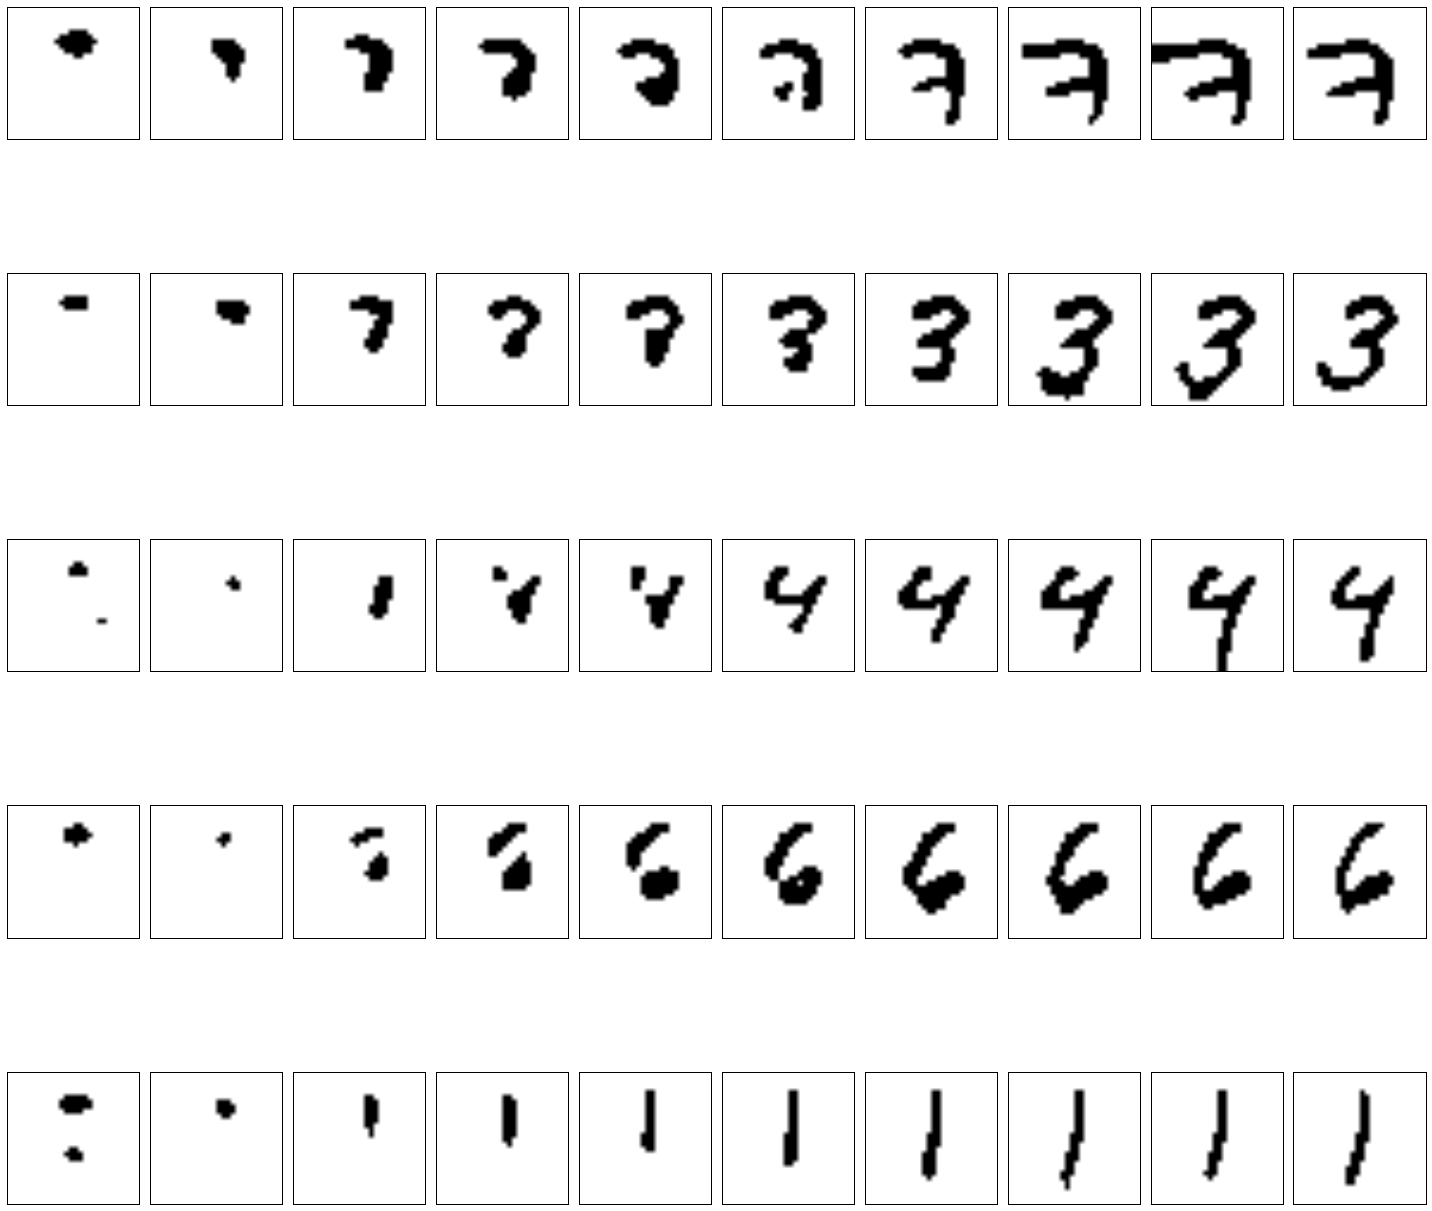
\includegraphics[width=0.35\textwidth]{images/draw_inference.png}
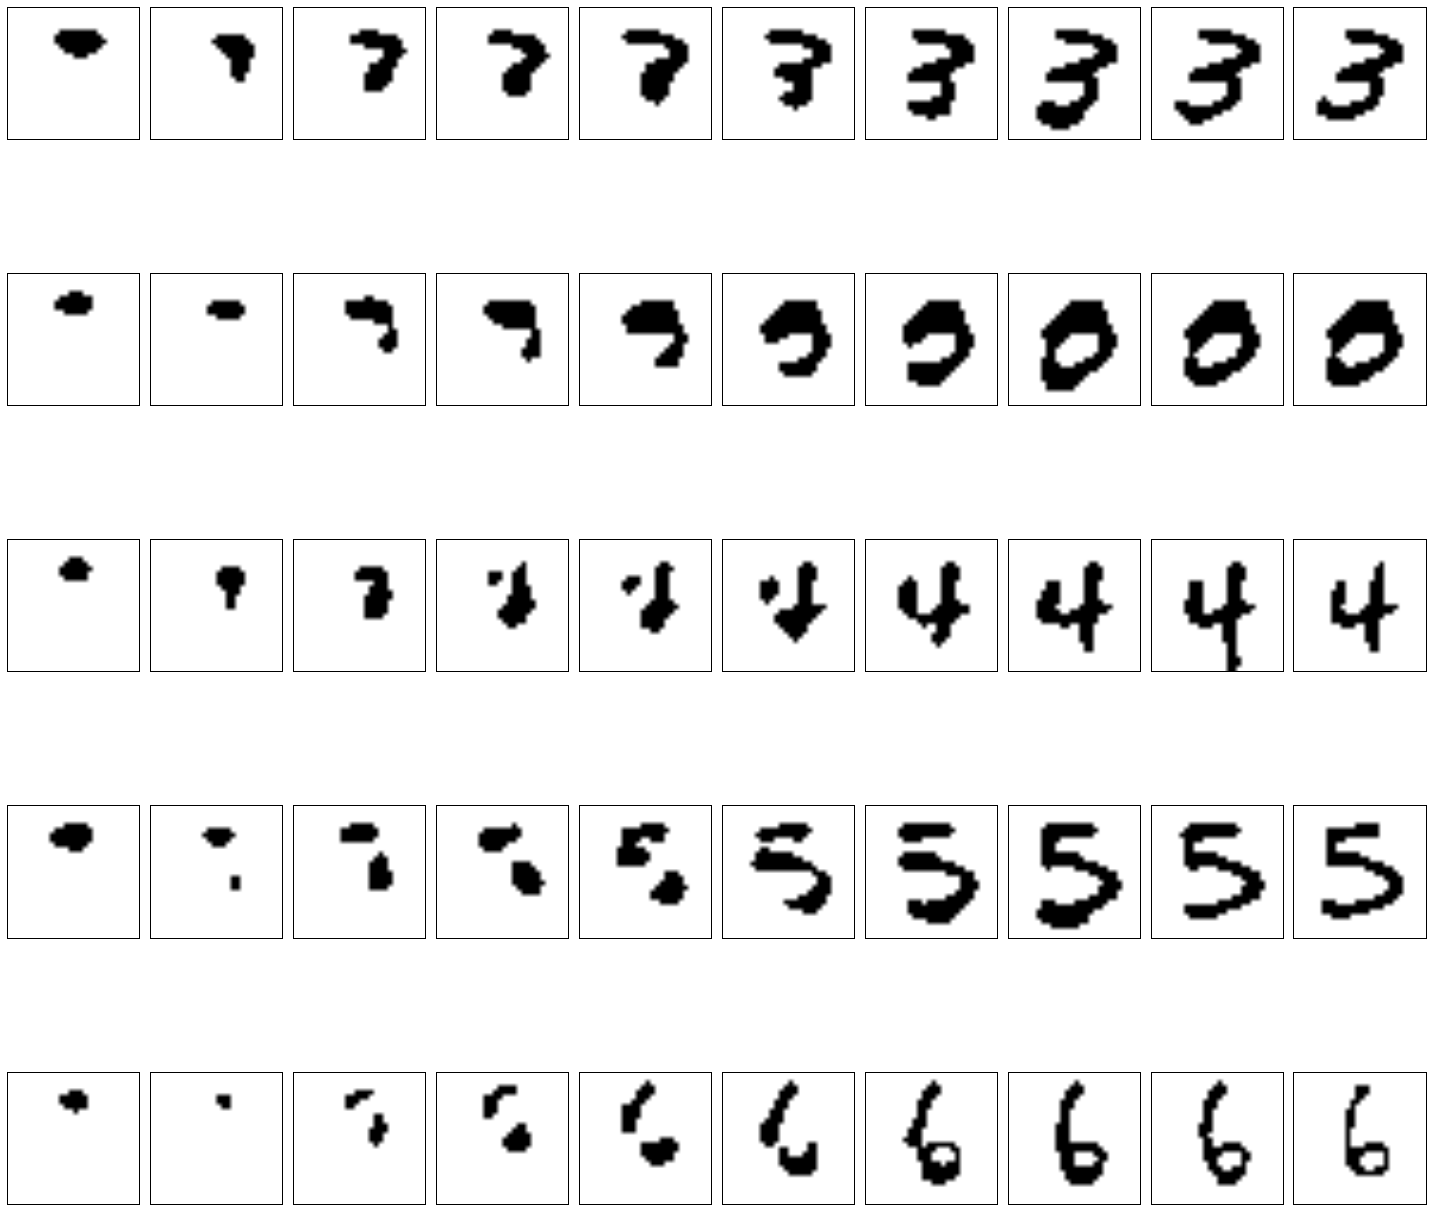
\includegraphics[width=0.35\textwidth]{images/draw_generate.png}
\caption{Images on the left are reconstructed by the real input images using DRAW. Images on the right are generated from random Gaussian input using DRAW. }
\label{figure:draw}
\end{figure}

\begin{figure}[!ht]
\centering
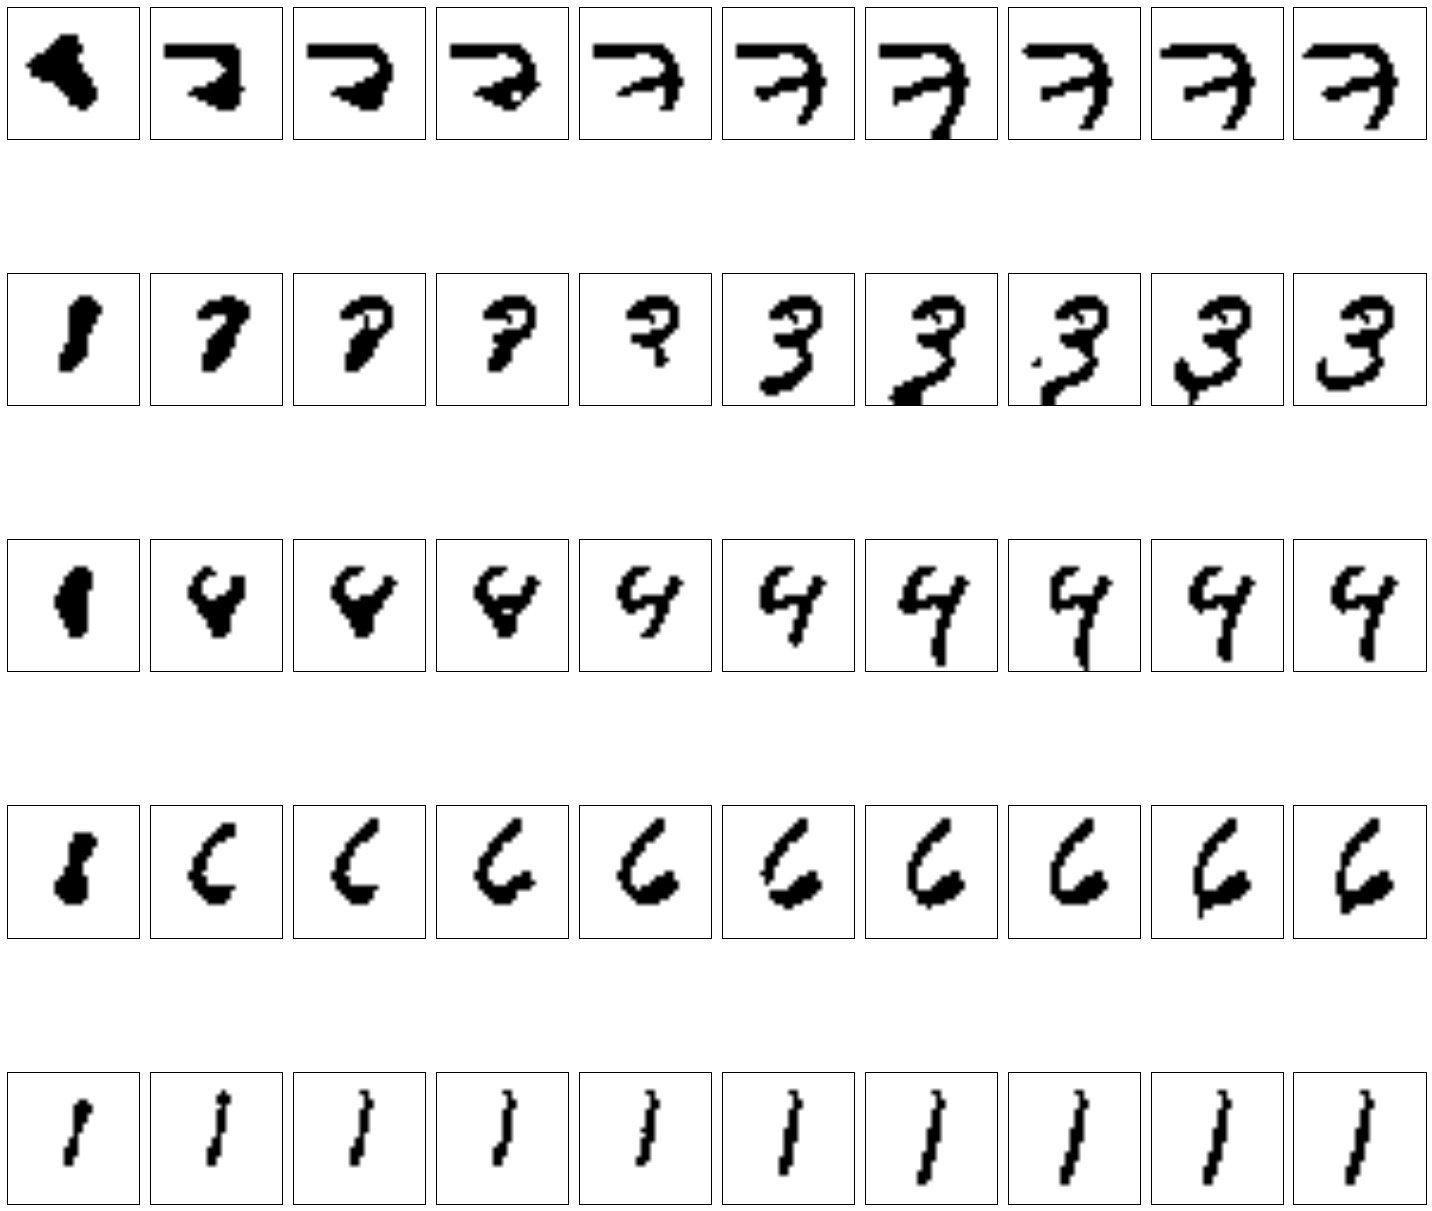
\includegraphics[width=0.35\textwidth]{images/drwa_gan_inference.png}
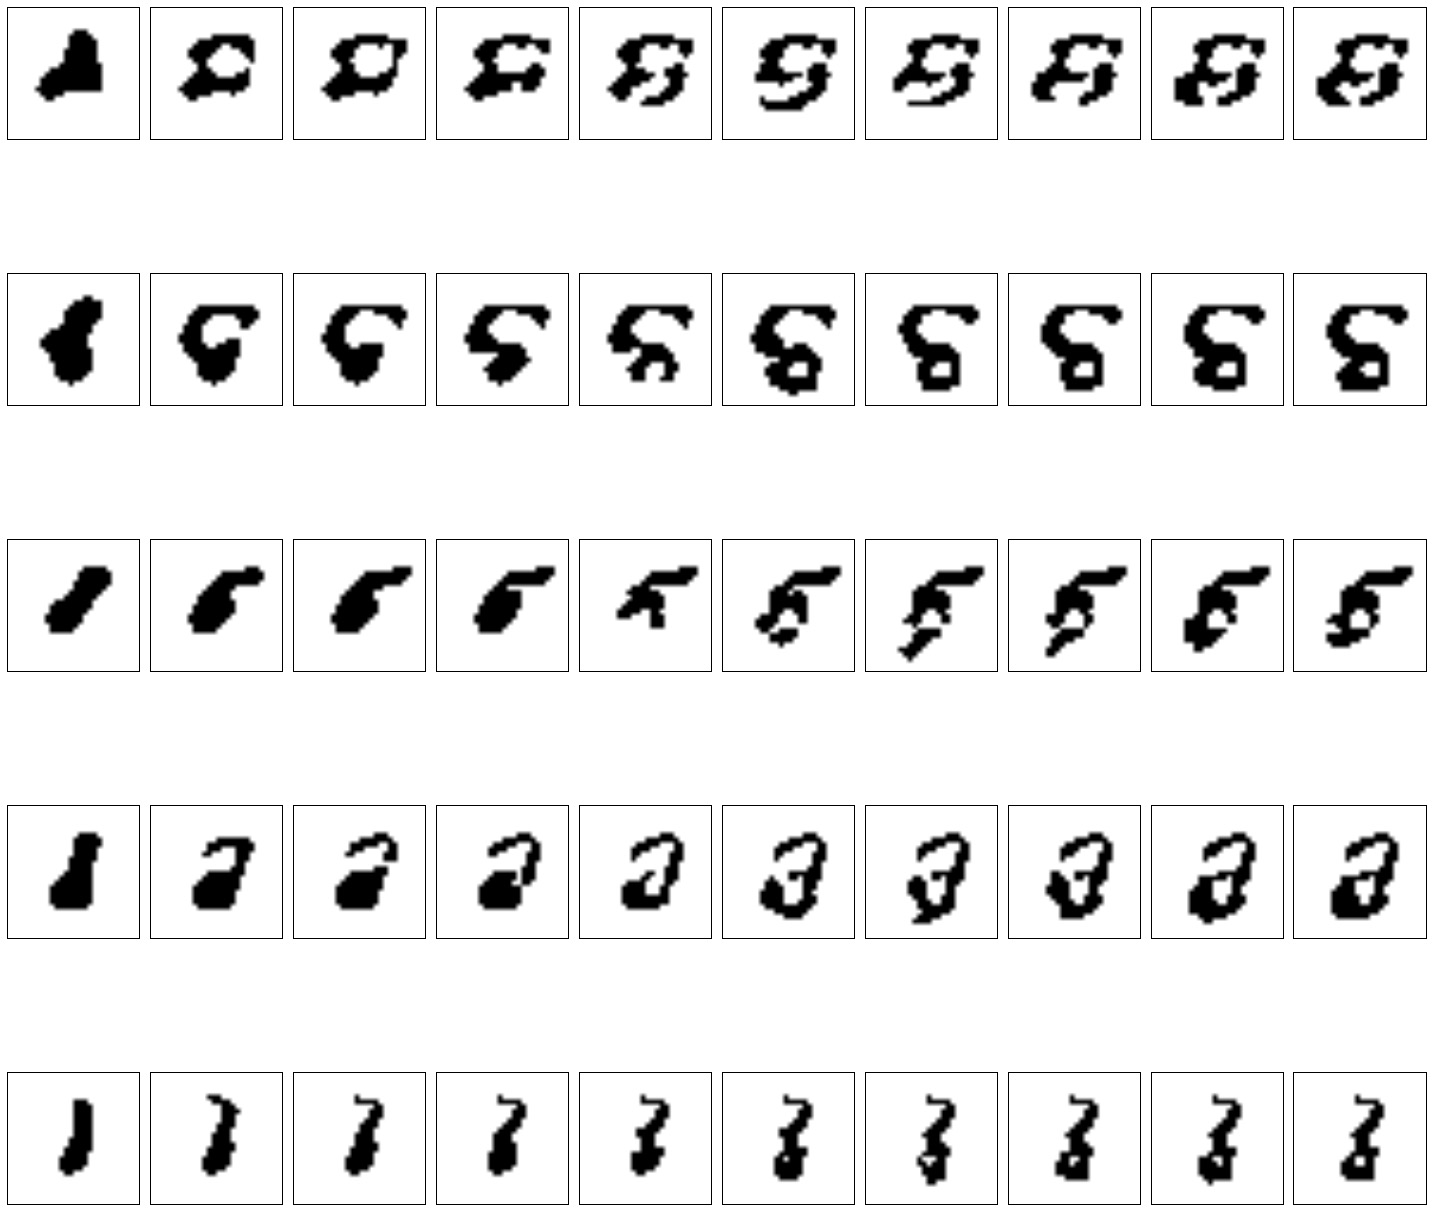
\includegraphics[width=0.35\textwidth]{images/draw_gan.png}
\caption{Images on the left are reconstructed by the real input images using DRAW-GAN. Images on the right are generated from random Gaussian input using DRAW-GAN. }
\label{figure:draw_gan}

\end{figure}

\section{Conclusion and Future Work}
Variational auto-encoders and generative adversarial networks are two promising classes of generative models which have their respective drawbacks. For example, VAEs generate blurry images while GANs are difficult to train and generate images which lack variaty. This work serves as an initiate of combining various variants of VAEs with GANs. In particular, we propose CVAE-GAN, SSL-VAE-GAN and DRAW-GAN. We also apply generative models to the problems of image completion, style transfer and semi-supervised learning. While CVAE-GAN generated better images than the baseline model CVAE, SSL-VAE-GAN and DRAW-GAN fail to achieve expected performance. We propose several potential solutions to these problems and leave them to future work.
\section{Lessons Learned}
\begin{itemize}
\item TensorFlow, although tricky to learn at first, became quite helpful when building more complicated models. In particular, the TensorFlow-Slim library allowed us to access standard neural network layers easily so that we did not have to manage weights and variables manually.

\item Some of the models were difficult to train, and batch normalization was critical to reduce sensitivity to hyperparameters (e.g. learning rate) and to help bring the loss down.
\item The pooling layer is not helpful in generateive models of images like VAEs and GANs.
\item Use a smaller learning rate (0.0001) to train GANs but use a higher one (0.001) to train VAEs.
\end{itemize}
\section{Team Contributions}

\begin{itemize}
\item Jianbo Chen (?\%): implemented VAE framework on which all other implementations are based, improved convolutional architecture, improved/implemented GAN-based models, contributed to poster, wrote report
\item Billy Fang (?\%): implemented CVAE (with digit generation, image completion, and style transfer), implemented SSL, implemented baseline GAN-based models, contributed to poster, wrote report
\item Cheng Ju (?\%): implemented and experimented with DRAW, conditional DRAW, DRAW with GAN. Build general DRAW object that has options to construct flexible combinations of DRAW variants (conditional/unconditional and vanilla/GAN), wrote report
\end{itemize}












\bibliographystyle{plain}
\bibliography{cs294_bib}

\nocite{*}

\end{document}
